\newpage
\subsection{Caso d'uso UC3: Login}
\label{UC3}
\begin{figure}
	\centering
	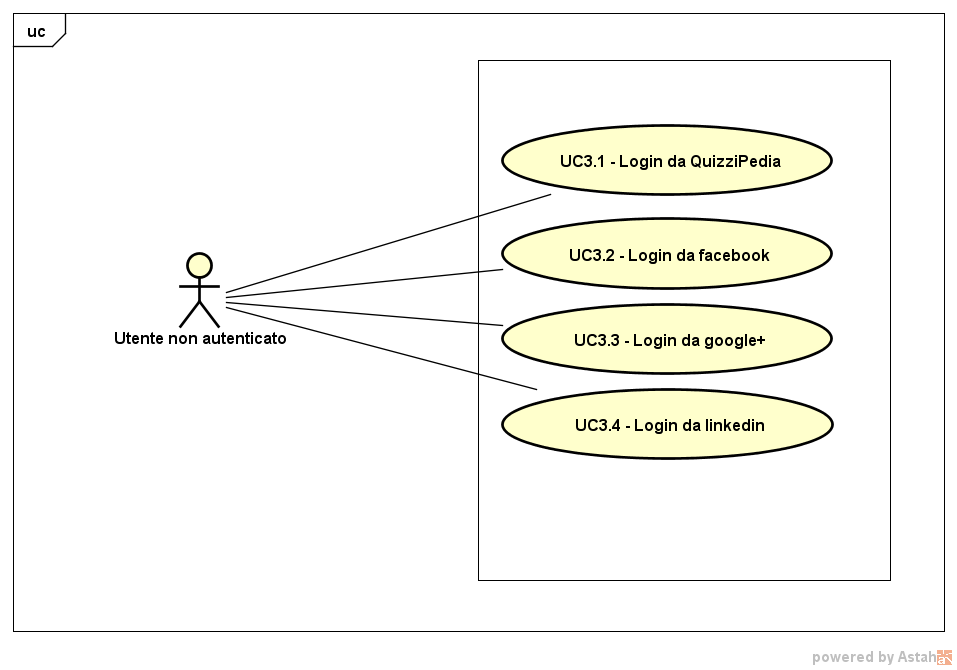
\includegraphics[scale=0.5]{UML/UC3.png}
	\caption{UC3: Login}
\end{figure}
\FloatBarrier
\begin{itemize}
	\item \textbf{Attori}: utente non autenticato;
	\item \textbf{Descrizione}: l'attore si può autenticare tramite uno dei metodi proposti;
	\item \textbf{Precondizione}: il sistema è avviato e pronto per l'utilizzo e mostra la pagina di login;
	\item \textbf{Postcondizione}: l'attore è autenticato;
	\item \textbf{Scenario principale}: l'attore sceglie uno dei seguenti modi per autenticarsi:
		\begin{itemize}
			\item L'attore può effettuare il login con \progetto (UC3.1);
			\item L'attore può effettuare il login con Facebook (UC3.2);
			\item L'attore può effettuare il login con Twitter (UC3.3);
			\item L'attore può effettuare il login con Google+ (UC3.4);
			\item L'attore può effettuare il login con Linkedin (UC3.5).
		\end{itemize}
\end{itemize}

\subsubsection{Caso d'uso UC3.1: Login da \progetto}
\label{UC3.1}
\begin{figure}
	\centering
	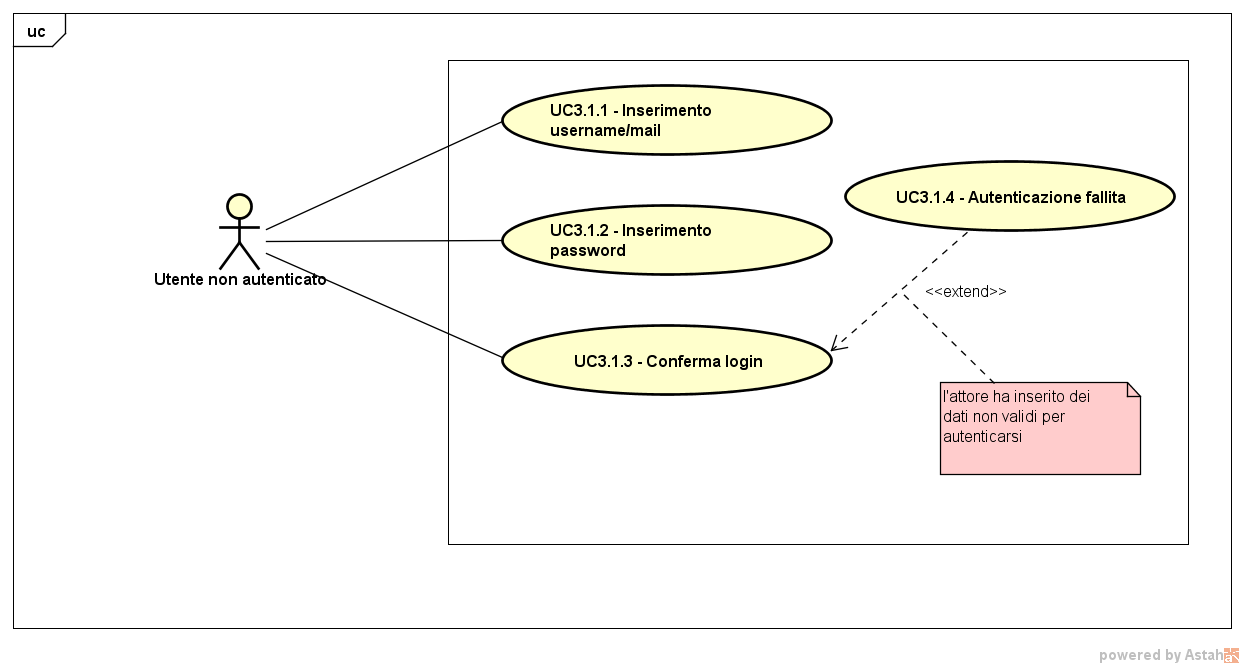
\includegraphics[scale=0.5]{UML/UC3_1.png}
	\caption{UC3.1: Login da \progetto}
\end{figure}
\FloatBarrier
\begin{itemize}
	\item \textbf{Attori}: utente non autenticato;
	\item \textbf{Descrizione}: l'attore si può autenticare inserendo username/mail e password, con cui è registrato;
	\item \textbf{Precondizione}: il sistema è avviato e pronto per l'utilizzo e mostra la pagina di login;
	\item \textbf{Postcondizione}: il sistema ha autenticato l'attore e quindi mostra all'attore autenticato la sua area riservata;
	\item \textbf{Scenario Principale}:
	\begin{itemize}
		\item L'attore può inserire l'username oppure la mail utilizzata al momento della registrazione (UC3.1.1);
		\item L'attore può inserire la password (UC3.1.2);
		\item L'attore può confermare il login (UC3.1.3).
	\end{itemize}
	\item \textbf{Estensioni}: autenticazione fallita (UC3.1.4).
\end{itemize}

\subsubsection{Caso d'uso UC3.1.1: Inserimento username/mail}
\begin{itemize}
	\item \textbf{Attori}: utente non autenticato;
	\item \textbf{Descrizione}: l'attore può inserire l'username o la mail associata al proprio account;
	\item \textbf{Precondizione}: il sistema presente all'attore lo spazio destinato a questa operazione;
	\item \textbf{Postcondizione}: l'attore ha inserito username/mail;
	\item \textbf{Scenario principale}: l'attore inserisce l'username o la mail associata al proprio account. 
\end{itemize}

\subsubsection{Caso d'uso UC3.1.2: Inserimento password}
\begin{itemize}
	\item \textbf{Attori}: utente non autenticato;
	\item \textbf{Descrizione}: l'attore può inserire la password associata al proprio account;
	\item \textbf{Precondizione}: il sistema presenta all'attore lo spazio destinato a questa operazione;
	\item \textbf{Postcondizione}: l'attore inserisce la password;
	\item \textbf{Scenario principale}: l'attore inserisce la password associata al proprio account.
\end{itemize}

\subsubsection{Caso d'uso UC3.1.3: Conferma login}
\begin{itemize}
	\item \textbf{Attori}: utente non autenticato;
	\item \textbf{Descrizione}: l'attore può confermare i dati inseriti per effettuare il login;
	\item \textbf{Precondizione}: l'attore ha inserito l'username/mail e la password;
	\item \textbf{Postcondizione}: l'attore è autenticato;
	\item \textbf{Scenario principale}: l'attore conferma i dati inseriti per effettuare la login con il proprio account.
\end{itemize}

\subsubsection{Caso d'uso UC3.1.4: Autenticazione fallita}
\begin{itemize}
	\item \textbf{Attori}: utente non autenticato;
	\item \textbf{Descrizione}: l'attore ha inserito dei dati non validi per autenticarsi, in particolare:
		\begin{itemize}
		\item L'attore inserisce un username inesistente;
		\item L'attore inserisce una mail non registrata;
		\item L'attore inserisce una password che non corrisponde a quella associata all'username/mail inserita;
		\item L'attore non inserisce una password;
		\item L'attore non inserisce né un username/mail né una password.
		\end{itemize}
	\item \textbf{Precondizione}: l'attore ha confermato il login;
	\item \textbf{Postcondizione}: il sistema avvisa l'attore dell'errore verificatosi tramite un opportuno messaggio;
	\item \textbf{Scenario principale}: l'attore visualizza un messaggio relativo ai dati errati che erano stati precedentemente inseriti.	
\end{itemize}

\subsubsection{Caso d'uso UC3.2: Login con Facebook}
\begin{itemize}
	\item \textbf{Attori}: utente non autenticato;
	\item \textbf{Descrizione}: l'attore può autenticarsi utilizzando Facebook;
	\item \textbf{Precondizione}: l'attore visualizza la pagina di login e sceglie la login con Facebook;
	\item \textbf{Postcondizione}: l'attore è autenticato;
	\item \textbf{Scenario principale}: l'attore effettua il login tramite Facebook.
\end{itemize}
\subsubsection{Caso d'uso UC3.3: Login con Twitter}
\begin{itemize}
	\item \textbf{Attori}: utente non autenticato;
	\item \textbf{Scopo e descrizione}: l'attore può autenticarsi utilizzando Twitter;
	\item \textbf{Precondizione}: l'attore visualizza la pagina di login e sceglie la login con Twitter;
	\item \textbf{Postcondizione}: l'attore è autenticato;
	\item \textbf{Scenario principale}: l'attore effettua il login tramite Twitter.
\end{itemize}
\subsubsection{Caso d'uso UC3.4: Login con Google+}
\begin{itemize}
	\item \textbf{Attori}: utente non autenticato;
	\item \textbf{Descrizione}: l'attore può autenticarsi utilizzando Google+;
	\item \textbf{Precondizione}: l'attore visualizza la pagina di login e sceglie la login con Google+;
	\item \textbf{Postcondizione}: l'attore è autenticato;
	\item \textbf{Scenario principale}: l'attore effettua il login tramite Google+.
\end{itemize}
\subsubsection{Caso d'uso UC3.5: Login con Linkedin}
\begin{itemize}
	\item \textbf{Attori}: utente non autenticato;
	\item \textbf{Descrizione}: l'attore può autenticarsi utilizzando Linkedin;
	\item \textbf{Precondizione}: l'attore visualizza la pagina di login e sceglie la login con Linkedin;
	\item \textbf{Postcondizione}: l'attore è autenticato;
	\item \textbf{Scenario principale}: l'attore effettua il login tramite Linkedin.
\end{itemize}